% !TEX encoding = UTF-8 Unicode
%Encoding: UTF-8

        
\section{Initial Situation}

\subsection{State of the Art} 
Abbreviations of \ac{ADAM} or \aclp{CNN} (\acsp{CNN}) are introduced here. Sections can be referenced by Sec. \ref{sec:appdix_main_script}, while tables and figures can be referenced the same way (see Tab. \ref{tab:table1} and Fig. \ref{fig:figure1} or Fig. \ref{fig:figure2}).

\begin{figure}[htb!]
 \centering
 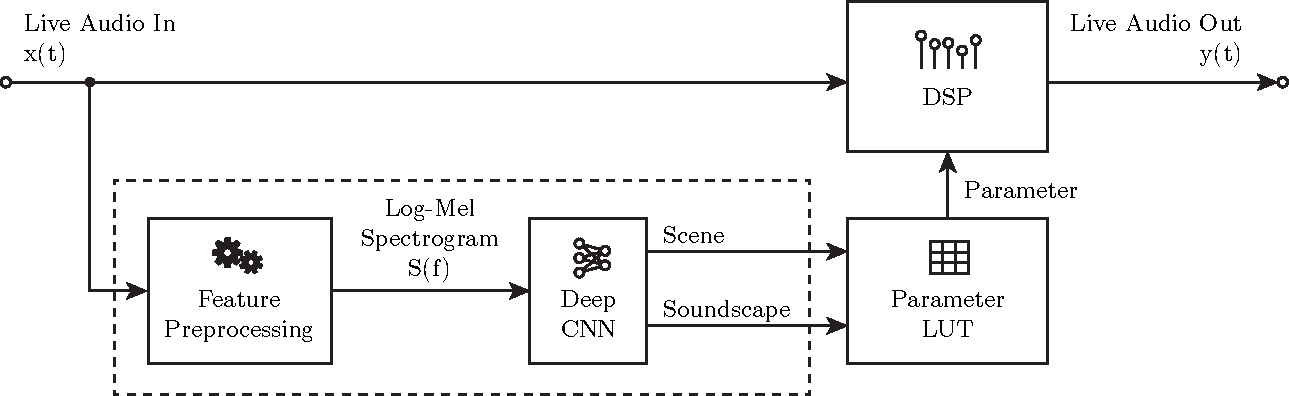
\includegraphics[width=0.85\textwidth]{01_Intended_System.pdf}
 \caption
 [Caption 1 in list of figures]
 {Caption 1 below figure \cite{axodraw}.}
 \label{fig:figure1}
\end{figure}

\begin{figure}[htb!]
 \centering
 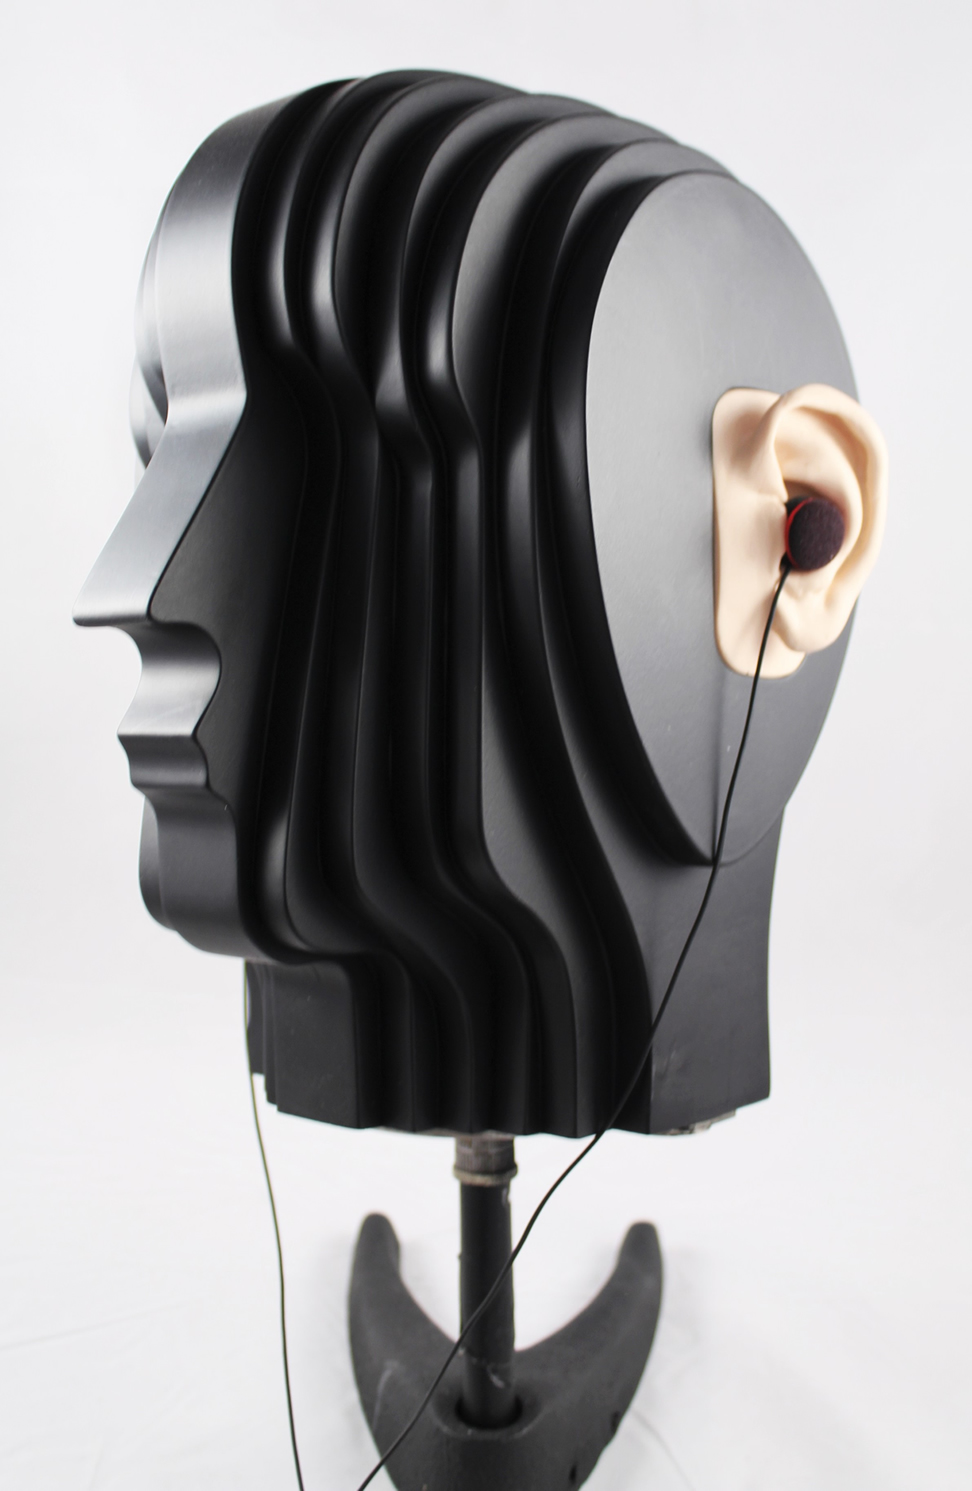
\includegraphics[width=0.15\textwidth]{02_DummyHead.jpg}
 \caption{Caption 2 below figure.}
 \label{fig:figure2}
\end{figure}

\subsection{Our Approach}


\newpage
\section{Project Scope}

\subsection{Time Horizon}

\subsection{Previous Work}

\subsection{Documentation Structure}
